\section{Use Case}
\begin{frame}{Riskprofiling}
	\begin{center}
		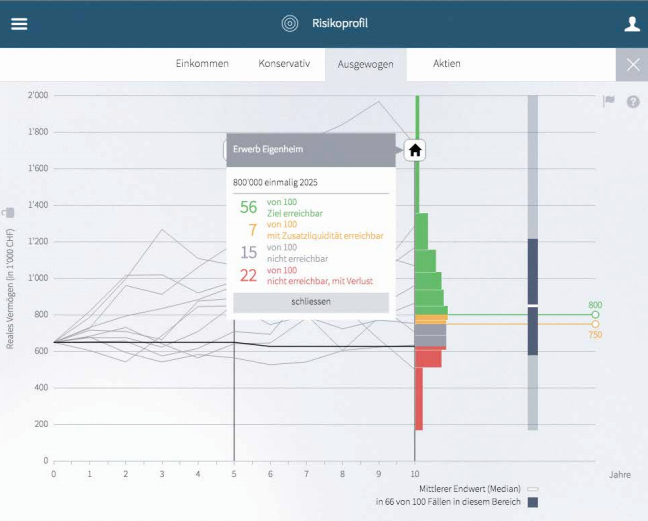
\includegraphics[width=0.8\textwidth]{risk-profiling}
	\end{center}
\end{frame}

\begin{frame}{Performance Improving prior Parallelization}
	\begin{itemize}
		\item A problem needs to be parallelizable
		\item Parallelization always adds complexity
		\item Maybe it's enough to improve \enquote{synchronous} code
	\end{itemize}
\end{frame}

\begin{frame}[plain]
	\begin{tikzpicture}
		\begin{axis}[
			mlineplot,
			width=1\textwidth,
			height=1\textheight,
			title=Execution Time for 100'000 runs,
			xlabel={Projects},
			ylabel={Mean in seconds},
			xmin=0,
			xmax=18,
			xtick={1, 4, 8, 16},
			ymin=0,
			ymax=2.8,
			legend entries={v1,v2,v3, v4, v5, v6, v7},
			legend style = { at = {(0.2,1.0)}},
			minor tick num=5,
			cycle list name=mylist cycle
		]
		\addplot table {../v1.data};
		\addplot table {../v2.data};
		\addplot table {../v3.data};
		\addplot table {../v4.data};
		\addplot table {../v5.data};
		\addplot table {../v6.data};
		\addplot table {../v7.data};
	\end{axis}
\end{tikzpicture}
\end{frame}

\begin{frame}{V1, authored by Micha Reiser}
	\begin{itemize}
		\item Computes the simulation result over 15 years
		\item For each project
		\begin{itemize}
			\item Creates the four groups \enquote{red, gray, yellow, green}
			\item Creates for each group 10 buckets and assigns the simulation values
		\end{itemize}
		\item Median, min, max are computed in the chart
	\end{itemize}
	
	\begin{alertblock}{Main Concern}
		Simulation returns all values instead of the needed information median, min and max. Therefore, absolutely unsuited for parallelization because of large data amount to be transferred.
	\end{alertblock}

\end{frame}

\begin{frame}{V2, only returns Information needed by Chart}
	\begin{itemize}
		\item Marginal Faster (no array resizes, $\approx 20$ms)
		\item Chart needs to perform less computations
		\item Easier to parallelize, less data needs to be transferred
	\end{itemize}
\end{frame}

\begin{frame}{V3, Address V8 deoptimizations}
	If you see this...
	
	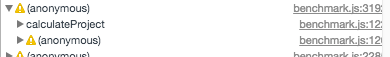
\includegraphics[scale=0.45]{deopt}
	
	... you are doomed ;)
\end{frame}

\begin{frame}{...or at least, there is much Room for Improvements}
	\begin{block}{V8 Optimization Killers~\cite{bluebird2017}}
		\begin{itemize}
			\item Unsupported Syntax (e.g. \javascriptinline/debugger/, \javascriptinline/eval/, \javascriptinline/with/, generator functions...) 
			\item Manipulating \javascriptinline/arguments/
			\item Very large Switch-case Statements (+128 cases)
			\item \javascriptinline/for in/
			\item Infinite Loops with deep logic or unclear exit
			\item Others
		\end{itemize}
	\end{block}
	
	\pause
	\begin{block}{Workaround}
		\begin{itemize}
			\item Clean Code
			\item Small Functions
		\end{itemize}	
	\end{block}
\end{frame}

\begin{frame}[fragile, shrink]{In this Case, the Reason is a Dynamic Object Structure}
	\begin{javascriptcode*}{highlightlines={18-20}, fontsize=\tiny}
const valuesByGroup: { [groupName: string]: number } = {};
const bucketSize = Math.round(simulatedValuesThisYear.length / NUMBER_OF_BUCKETS);
const buckets: IBucket[] = [];

for (let i = 0; i < simulatedValuesThisYear.length; i += bucketSize) {
	const bucket: IBucket = {
		max: Number.MIN_VALUE,
		min: Number.MAX_VALUE,
		subBuckets: {}
	};

	for (let j = i; j < i + bucketSize; ++j) {
		const value = simulatedValuesThisYear[j];
		bucket.min = Math.min(bucket.min, value);
		bucket.max = Math.max(bucket.max, value);

		const group = groupForValue(simulatedValuesThisYear[j], groups);
		valuesByGroup[group.name] = (valuesByGroup[group.name] || 0) + 1;
		const subBucket = bucket.subBuckets[group.name] = bucket.subBuckets[group.name] || 
						{ group: group.name, max: Number.MIN_VALUE, min: Number.MAX_VALUE };
		subBucket.min = Math.min(subBucket.min, value);
		subBucket.max = Math.max(subBucket.max, value);
	}

	buckets.push(bucket);
}
	\end{javascriptcode*}

\end{frame}

\begin{frame}{...that makes it Impossible to Optimize the Property Access}
	\begin{center}
		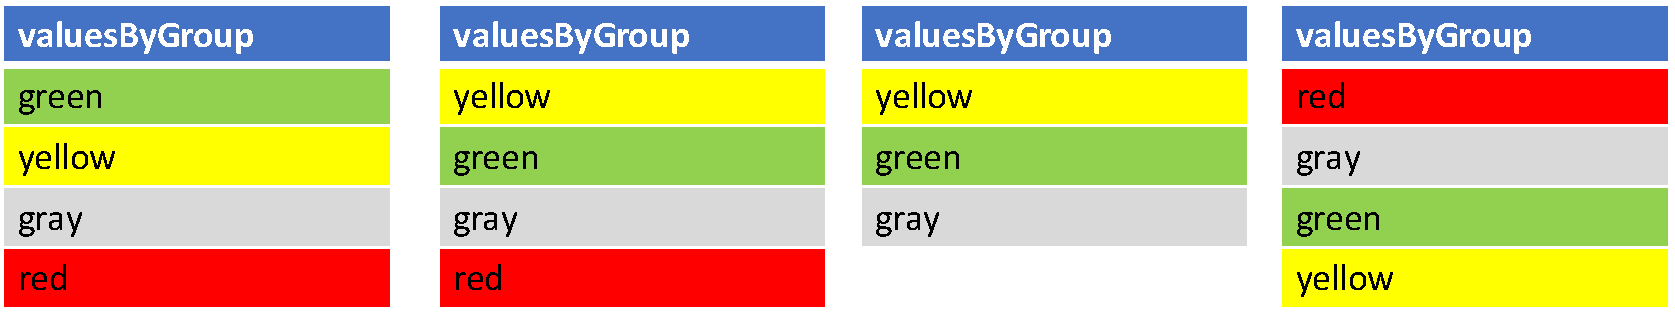
\includegraphics[width=1\textwidth]{memory-model}
	\end{center}
	
	Depending on the order of the simulated values the offset for the properties differ, e.g. for \enquote{green}:
	
	\begin{enumerate}[<+->]
		\item +0
		\item +4 (32bit pointer)
		\item +4
		\item +8
		\item ...
	\end{enumerate}
	
	\only<6>{Therefore, V8 deoptimizes the \textbf{whole} function}
\end{frame}

\begin{frame}[fragile, shrink]{Solution: Ensure that the Object is always Initialized in the same Order}
	\begin{javascriptcode}
const bucket: IBucket = {
	max: Number.MIN_SAFE_INTEGER,
	min: Number.MAX_SAFE_INTEGER,
	// Needed to avoid deoptimization because of changed attribute orders in subBuckets. Initialize with const order
	subBuckets: {
		green: {
			group: "green",
			max: Number.MIN_SAFE_INTEGER,
			min: Number.MAX_SAFE_INTEGER,
			empty: true
		},
		yellow: {
			group: "yellow",
			max: Number.MIN_SAFE_INTEGER,
			min: Number.MAX_SAFE_INTEGER,
			empty: true
		},
		//...
	}
};	
	\end{javascriptcode}
\end{frame}

\begin{frame}{This small Change Improves Performance by up to 235ms}
	\begin{tikzpicture}
		\begin{axis}[
			mlineplot,
			width=1\textwidth,
			height=1\textheight,
			title=Execution Time for 100'000 runs,
			xlabel={Projects},
			ylabel={Mean in seconds},
			xmin=0,
			xmax=18,
			xtick={1, 4, 8, 16},
			ymin=0,
			ymax=2.8,
			legend entries={v1,v3},
			legend style = { at = {(0.2,1.0)}},
			minor tick num=5,
			cycle list name=mylist cycle
		]
		\addplot table {../v1.data};
		\addplot table {../v3.data};
	\end{axis}
\end{tikzpicture}
\end{frame}

\begin{frame}{Further Improvements}
	\begin{itemize}
		\item v4: Reduce Nesting of Functions (-47ms)
		\item v5: Create Arrays with expected Size (-60ms)
		\item v6: Only simulate number of Years needed (-270ms)
		\item v7: Avoid Object Destructuring (-61ms)
	\end{itemize}
	
	\begin{block}{Overall}
		Improvement by 666ms in best case (1.76 instead of 2.426s) or by 28\%
	\end{block}

\end{frame}

\begin{frame}{Further Improving the Performance by Parallelizing the Computation}
	\begin{itemize}[<+->]
		\item Computation consists of
			\begin{itemize}
				\item Simulation
				\item Creating Buckets for each Projects
			\end{itemize}
		\item Parallelization by computing buckets for multiple projects simultaneous 
		\item However, simulation is most expensive
		\item But sharing the data of the simulation between worker is as expensive as performing the simulation in each worker
		\item So it only makes sense to parallelize if there are 2+ projects
	\end{itemize}
	
	\only<8>{\begin{block}{But Performance is not everyting}
		The UI is no longer blocked for $\approx 2$s
	\end{block}}

\end{frame}

\begin{frame}{Performance Improvement of up to 300ms (2 Cores, HT)}
	\begin{tikzpicture}
		\begin{axis}[
			mlineplot,
			width=1\textwidth,
			height=0.8\textheight,
			title=Execution Time for 100'000 runs,
			xlabel={Projects},
			ylabel={Mean in seconds},
			xmin=0,
			xmax=18,
			xtick={1, 4, 8, 16},
			ymin=0,
			ymax=2.8,
			legend entries={v1,v7, transpiled},
			legend style = { at = {(0.3,1.0)}},
			minor tick num=5,
			cycle list name=mylist cycle
		]
		\addplot table {../v1.data};
		\addplot table {../v7.data};
		\addplot table {../transpiled.data};
	\end{axis}
\end{tikzpicture}

But sometimes it is even slower.

\end{frame}
